\chapter{Simulation}

Simulating the robot in sample environments allows for more rapid algorithmic development and excludes implementation details which may masquerade as errors in the algorithm. The simulation was written in MATLAB for this project. 
The simulation constructed a virtual environment using line segments and approximated the robot as a point on the plane. 
A simple kinematic model of the robot is used, as modeling the full kinematics of the Nao robot is not necessary for the efficacy of the algorithm. A basic approximation for inertia is made by low pass filtering all velocity commands. Motion noise is injected by adding uniform random noise to the linear and angular velocities. The resultant velocities are integrated to gain robot position using a first order approximation.
The sonar beams are approximated as cones in the plane with the sensor model returning the distance to the closest object within the region of the cone. These ranges are also perturbed by uniform random noise before being returned to the navigation algorithm.
The goal location is a randomly generated point in the map whose location the robot was aware of at all times.

\begin{figure}[h]
	\centering
	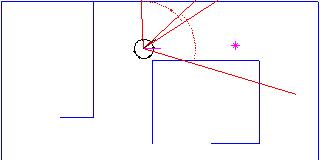
\includegraphics{sim_fig1.jpg}
	\caption[Planar robot simulation example.]
	{Planar robot simulation example. The robot is indicated by a black circle with the red cones simulating ultrasonic sensor beams and their detected range indicated by dotted red arcs in the red cone. Blue lines represent obstacles. The magenta line points towards the goal location, which is indicated by a magenta star.}
	\label{fig:simFig1}
\end{figure}

\section{Kinematics}
As the motion API for the Nao allowed commanding forward and angular velocities, the simple model used assumed that at each time step integration of these velocities would move the robot along the plane. Uniform random noise is added to these velocities to account for errors in encoding and motion. Dampening is added to simulate inertia in the robot's motion as a simple low pass filter. \\
\lstset{language=Matlab}
\begin{lstlisting}
	%%% MOTION NOISE %%%
	v = v + .2*rand(1);
	om = om + .01*rand(1);
	    
	%%% MOTION DAMPENING %%%
	v = 0.1*v + 0.9*vp;
	om = 0.1*om + 0.9*omp;
	   
	%%% MOTION MODEL %%%
	r_pose(3) = r_pose(3) + om*dt;
	r_pose(1) = r_pose(1) + v*cos(r_pose(3));
	r_pose(2) = r_pose(2) + v*sin(r_pose(3));
\end{lstlisting}
\lstinline$v, om, vp, omp$ are the current linear and angular velocities commanded by the path planning algorithm and the previous linear and angular velocities passed to the motion model, respectively. \lstinline$r_pose$ is a vector of the current x, y, $\theta$ of the robot in the plane. \lstinline$rand(1)$ generates a uniform random scalar between zero and one.

\section{Sensor Model}
The sensor model assumes that a single distance measurement should be returned which represents the range to the closest point on an occlusion in the sensor's field of view.
It uses parameterized line segments transformed into the robot's frame as obstacles. Using closed form equations, it iterates through every object in the map and checks for several conditions on each object to find the closest point on that object within the field of view of the sonar and then returns the distance to the closest object in that sonar cone.

\begin{figure}[h]
	\centering
	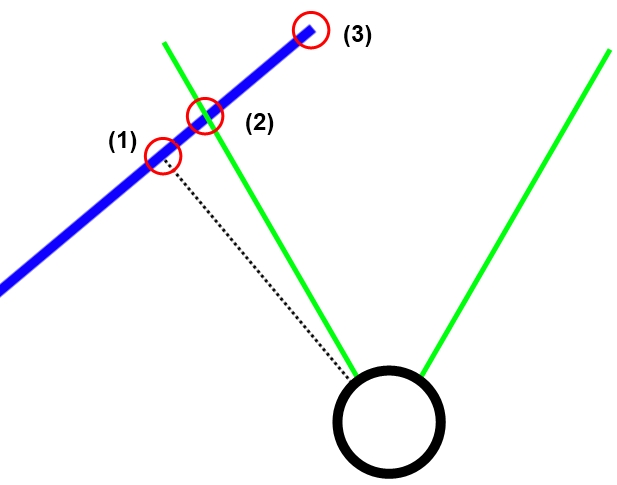
\includegraphics[width=0.5\textwidth]{sonar3.jpg}
	\caption[Sonar model points.]
	{Sonar model points. The robot is indicated by a black circle with the green lines representing the field of view of the sonar beam. The blue line represents the line segment object and the red circles indicate the three points the sonar model calculates. 1) is the perpendicular point on the occlusion, 2) the intersection between the line segment and the beam edge, 3) the end points of the line segment.}
	\label{fig:sonar3}
\end{figure}

Using infinite projections of the line segments, the points calculated are: 
\begin{enumerate}
	\item The perpendicular point on the line to the robot.
	\item The beam edge intersection with the line.
\end{enumerate}
These points were checked to be within the sonar cone and on the segmented line. Lastly, the if one of the segment's endpoints was in the sonar beam it too was considered. These points were all compared and the closest one was added to the range candidates for that beam. Once all the segments in the map were checked, the closest candidate was returned. Details of this model can be seen in the function \lstinline$getRangeBeam$ in Appendix \ref{sec:sensor_model}.

\section{GODZILA Path Planner}

Using the closed form solution for the cost functions, various force functions are used for the occlusions, goal, and inertia.
Occlusion force magnitudes are generated according to an inverse square and then applied to the direction vector along the orientation of the respective sensor in the robot's frame.

\begin{lstlisting}
	f_range1 = -1/(RANGE_COEFF*((ranges(1) - RANGE_OFF)^2))*[cos(-base_angle),sin(-base_angle)]';
	f_range2 = -1/(RANGE_COEFF*((ranges(2) - RANGE_OFF)^2))*[cos(base_angle),sin(base_angle)]';
	f_ranges = f_range1 + f_range2;
\end{lstlisting}
\lstinline$RANGE_COEFF$ and \lstinline$RANGE_OFF$ were experimentally determined constants used to prescribe the rate at which the robot is repelled from occlusions and a distance for which the robot is asymptotically repelled from. \lstinline$base_angle$ and \lstinline$ranges$ are the orientation of the ultrasonic sensor and a vector of the returned ranges from the sensors. Despite the actually orientation of the sensors with respect to the robot (25 degrees), the base angle of the sensors in simulation and on the robot used was 45 degrees. When the actual angle was used, the robot had a difficult time navigating between obstacles. When this was changed to 45 degrees, both the simulation and the actual robot are able to traverse more narrow apertures more easily.

The goal force is calculated using a similar inverse square law. The range is calculated, as the goal location is generated in the world frame, and then applied to the inverse square as a min between the range and some maximum value, so that the influence of the goal never gets too small. This is then brought into the robot frame.

\begin{lstlisting}
	goal_range = sqrt((r_pose(1) - goal(1))^2 + (r_pose(2) - goal(2))^2);
	f_goal = (1/((0.5*min(goal_range,25000))^2))*[goal(1) - r_pose(1), goal(2) - r_pose(2)]';
	f_goal = [cos(-r_pose(3)),-sin(-r_pose(3));sin(-r_pose(3)),cos(-r_pose(3))]*f_goal;
\end{lstlisting}
As the inertia force was always in the direction of the current heading, it takes the form of a constant.

\begin{lstlisting}
	f_heading = 0.01*[cos(0),sin(0)]';
\end{lstlisting}
The forces are then summed and the resultant orientation vector converted into an angular rate. 

\begin{lstlisting}
	f = f_ranges + f_goal + f_heading;
	th_in = (atan2(f(2),f(1)));
	om = TURN_MAGNITUDE*th_in*dt;
\end{lstlisting}
\lstinline$TURN_MAGNITUDE$ was an experimentally determined constant and \lstinline$dt$ is the time step used in the simulation.

The forward velocity is calculated in such a way that the robot will slow down when close to occlusions and speed up when far away. the $log$ function is used for this so the robot will not go too fast when obstacles are very far away. It also causea the robot to push exponentially harder away from walls if it gets too close. The $exp$ component slows the forward velocity when the robot has a large angular velocity. Finally, it is low passed with the previous forward velocity \lstinline$vp$.

\begin{lstlisting}
	v_desired = 0.75*log(min(ranges)/30)*(5*exp(-om));
	v = 0.1*vp + 0.9*v_desired;
\end{lstlisting}

A crude randomizer for trap detection was implemented using the variance of the naively integrated pose of the robot.

\section{Results}

Figure \ref{fig:sim_plots1} show some results of the simulation in various environments using randomized start and goal locations. This figure shows the algorithm was effective at driving the robot to the goal.

\begin{figure*}[htb]
	\centerline{
  		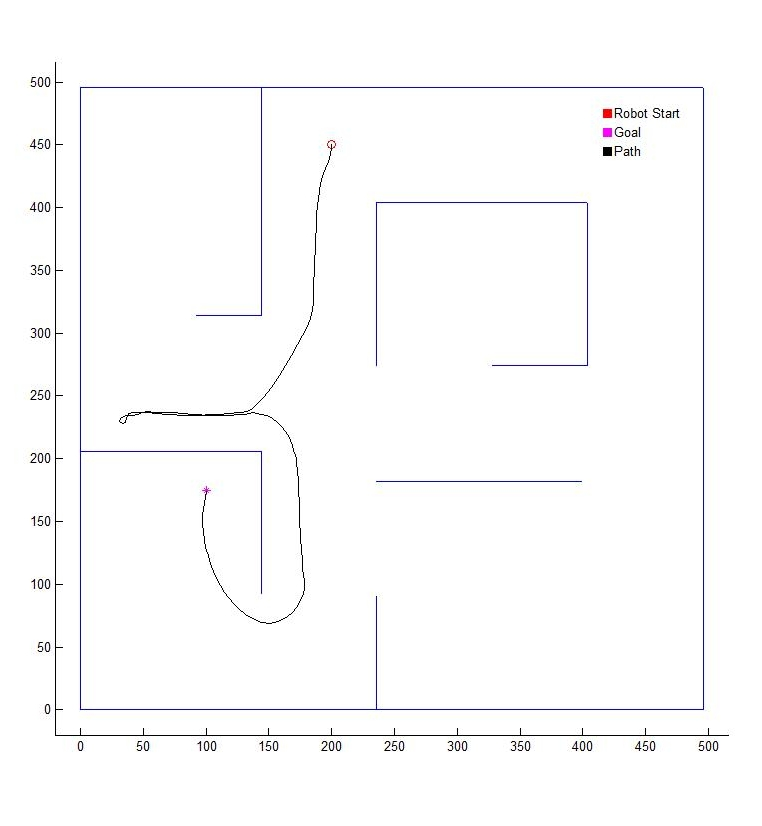
\includegraphics[width=0.5\textwidth,trim=0.2in 0.2in 0.2in 0.2in,clip=true]{path1.jpg}
  		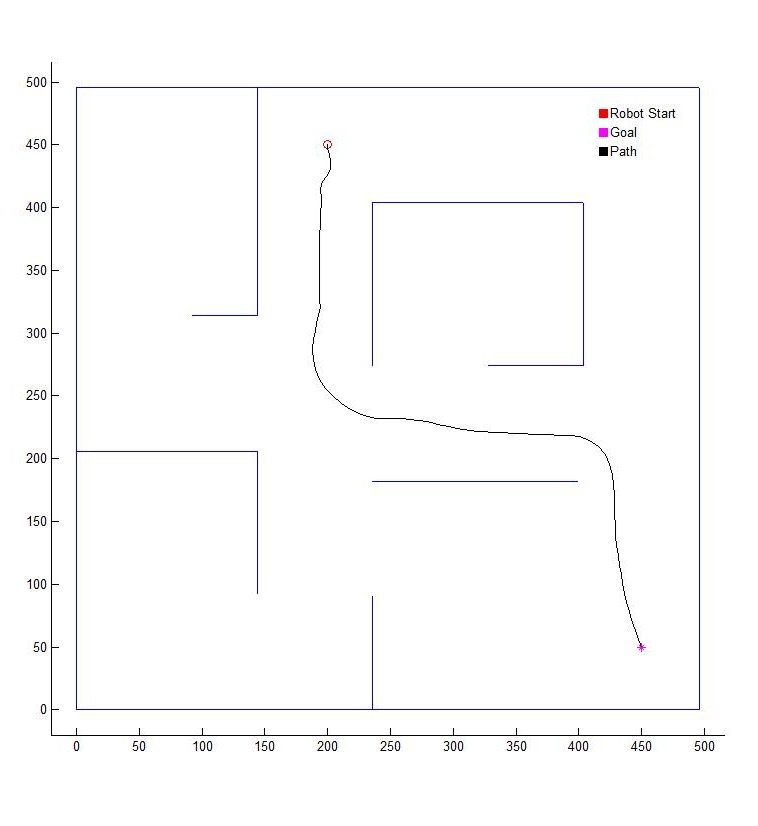
\includegraphics[width=0.5\textwidth,trim=0.2in 0.2in 0.2in 0.2in,clip=true]{path2.jpg}
  	} 
	\centerline{
		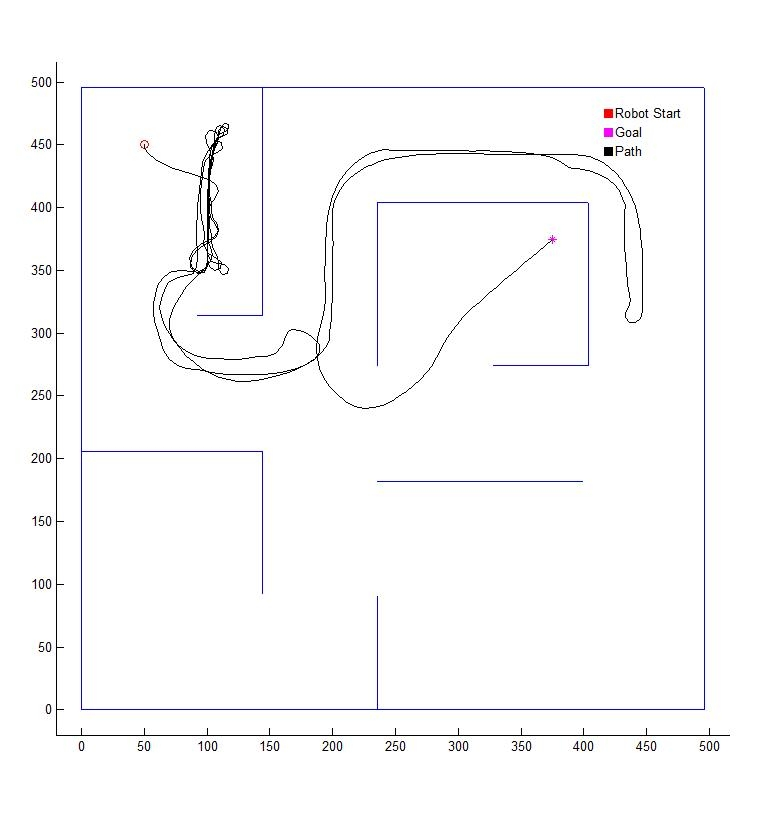
\includegraphics[width=0.5\textwidth,trim=0.2in 0.2in 0.2in 0.2in,clip=true]{path5.jpg}
        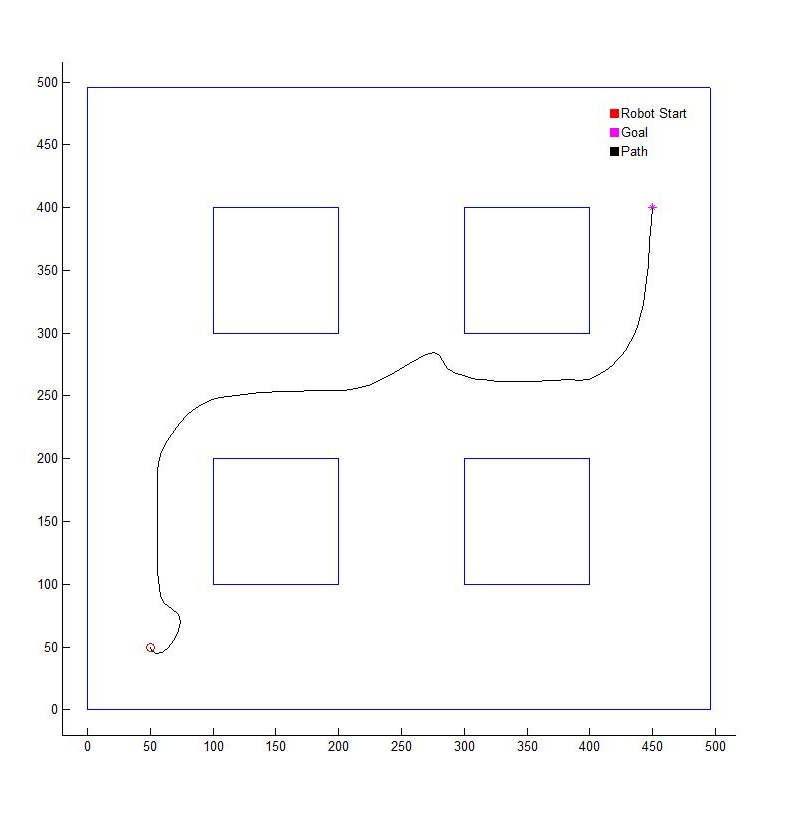
\includegraphics[width=0.5\textwidth,trim=0.2in 0.2in 0.2in 0.2in,clip=true]{path4.jpg}
    } 
    \caption[Simulation results.]
    {Simulation results. In these figures, the robot start and goal locations are shown in red and magenta, respectively. The trajectory of the robot is shown as a black line. The obstacles in the environment are shown as blue lines. The $X$ and $Y$ axis dimensions in the figures are in cm. Due to the large angular uncertainty inherent in the ultrasonic sensor measurements, some amount of meandering can be sometimes seen (as in the figure on the bottom left); however, the detection of local minima (or traps) and subsequent random walk components built into GODZILA ensure that the robot eventually finds a path to the goal location.}
    \label{fig:sim_plots1}
\end{figure*}




